% ----
% Criação do documento com a classe abntex2
% ----
\documentclass[a4paper, article, 12pt, openany, oneside, english, brazil]{abntex2}

% ---
% Pacotes fundamentais
% ---
\usepackage{times}			% Usa a fonte Latin Modern
\usepackage[T1]{fontenc}		% Seleção de códigos de fonte.
\usepackage[utf8]{inputenc}		% Codificação do documento (conversão automática dos acentos)
\usepackage{indentfirst}		% Indenta o primeiro parágrafo de cada seção.
\usepackage{color}		        % Controle das cores
\usepackage{graphicx}			% Inclusão de gráficos/figuras.
\usepackage{subcaption}			% Inclusão de subfiguras.
\usepackage{microtype} 			% para melhorias de justificação
\usepackage{amsmath}			% Pacote matemático
\usepackage[brazil]{babel}

% ---

% ---
% Pacotes de citações
% ---
% \usepackage[brazilian,hyperpageref]{backref}	 % Paginas com as citações na bibl
\usepackage[alf]{abntex2cite}	                 % Citações padrão ABNT


% % ----
% % Configurações dos pacotes
% % ----
% % Configurações do pacote backref
% % Usado sem a opção hyperpageref de backref
% \renewcommand{\backrefpagesname}{Citado na(s) página(s):~}
% % Texto padrão antes do número das páginas
% \renewcommand{\backref}{}
% % Define os textos da citação
% \renewcommand*{\backrefalt}[4]{
% 	\ifcase #1 %
% 		Nenhuma citação no texto.%
% 	\or
% 		Citado na página #2.%
% 	\else
% 		Citado #1 vezes nas páginas #2.%
% 	\fi}%
% % ---


% ---
% Informações de dados para CAPA e FOLHA DE ROSTO
% ---
\autor{Phelipe Teles da Silva}
\titulo{Determinantes macroeconômicos do spread bancário brasileiro (2011-2018)}
\data{2019}
\instituicao{Universidade Federal Rural do Rio de Janeiro}
\local{Seropédica, Rio de Janeiro}
\orientador[Orientadora:]{Débora Pimentel}
%\preambulo{}
%\tipotrabalho{}

\graphicspath{{../graficos/}}

\frenchspacing
% \setlength\afterchapskip{\lineskip}

\begin{document}
% ---
% Capa e Folha de Rosto
% ---
\imprimircapa
\imprimirfolhaderosto

% ---
% Insere o sumario automático
% ---
\pdfbookmark[0]{\contentsname}{toc}
\tableofcontents*
\cleardoublepage

\textual

\section{Introdução}

    O spread bancário tem sido de particular interesse para pesquisadores no Brasil, devido à peculiaridade de ser um dos maiores do mundo, o que pode ser visualizado na Figura \ref{spreadal}. Nela, podemos ver os maiores spreads bancários da América Latina, saltando à vista a liderança do Brasil por uma larga margem.

\begin{figure}[h]
  \centering
    \caption{Top 10 spreads bancários da América Latina em 2017}
      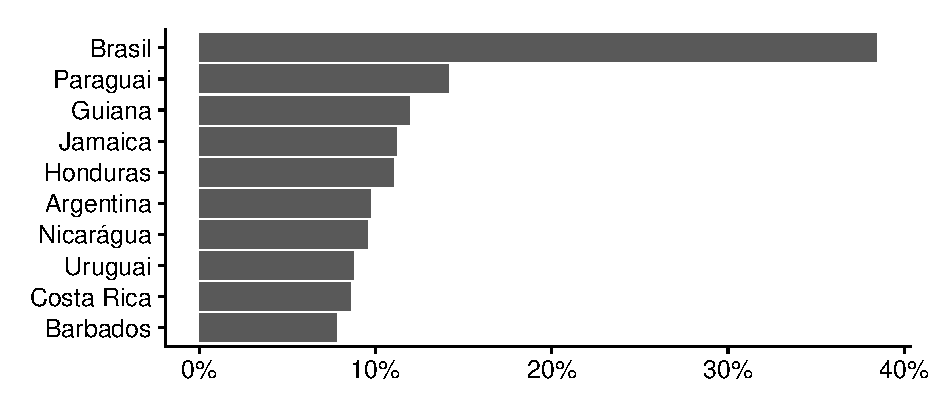
\includegraphics[width = 0.9\textwidth, scale=1]{spread_AL.pdf}
      \legend{Fonte: indicador ``FR.INR.LNDP'' do World Bank. Elaboração própria}
      \label{spreadal}
\end{figure}
    
    Com a bem-sucedida estabilização macroeconômica levada a cabo pelo Plano Real, esperava-se que esse nível finalmente começasse a convergir para os padrões internacionais mas, embora ele tenha de fato caído bastante, ainda continuou em um patamar relativamente bastante elevado.

    Desde então, uma das principais razões a que se vem atribuindo a isso é a política monetária, conduzida sob o Regime de Metas de Inflação (RMI) desde 1999, de manter a taxa básica de juros a níveis bastante elevados, com o objetivo de controlar a inflação. O spread, por ser, do ponto de vista ex-ante (ou antes do resultado financeiro das operações do banco), a diferença entre a taxa pela qual o banco empresta e a taxa pela qual ele capta recurso, a taxa básica de juros influencia diretamente o spread por representar um custo de oportunidade para a operação de crédito, visto que a Selic serve como indexador de parte dos títulos da dívida brasileira, uma aplicação muito menos arriscada e mais líquida que o crédito \cite[p.~7]{manhica12}.

    Mais recentemente, o debate foi reanimado devido à persistente queda da taxa Selic, trazendo consigo a expectativa de queda também do spread. Embora essa queda tenha mesmo se efetivado, seu ritmo foi tido como insatisfatório pelas autoridades \cite{valor1}. Há um elenco de fatores que podem ajudar a explicar isso, de variáveis micro, como a concorrência, assimetrias de informação sobre os tomadores de crédito e capacidade de recuperação de garantias\footnote{Ver \cite[p.~13]{reb2018}.}, a macroeconômicas, como a inadimplência e concentração bancária\footnote{Ver \cite{valor2}}.
    
    Em um cenário de incerteza macroeconômica, é interessante que se investigue os determinantes macroeconômicos do spread bancário, a fim de, com um melhor entendimento do caso brasileiro, contribuir para a efetividade das políticas de redução do spread, o que se apresenta ainda mais importante na atual situação de estagnação econômica, já que um spread mais baixo poderia ajudar na retomada, ao facilitar o acesso ao crédito dos agentes econômicos e, portanto, a realização de investimentos \cite[p.~8]{manhica12} além de, de modo geral, significar um sistema financeiro mais desenvolvido, com mais eficiência na intermediação financeira.


\section{Problema}

    Quais os principais determinantes macroeconômicos do spread bancário brasileiro?

\section{Hipótese}
    
    Seguindo a linha de \citeonline{afanasieff02}, em que se chega à conclusão de que as variáveis macroeconômicas são mais importantes que as microeconômicas para explicar a variação do spread ex-ante, foi feita a seleção das consideradas principais, com base na literatura. A seguir, uma descrição do que se pode esperar na estimação de suas relações com o spread.

    Espera-se um sinal positivo da taxa básica de juros (SELIC), por representar um custo de oportunidade para a operação de crédito; da inadimplência, pelo efeito risco de crédito; da inflação, porque dela os bancos se protegem via spread; do compulsório, por fazer parte dos custos de intermediação e, por fim, da concentração bancária devido ao efeito poder de mercado. Já o sinal esperado para a variável de atividade econômica é incerto, já que, por um lado, pode ser positivo devido à maior demanda por empréstimos, ou negativo se o aumento da escala da operação levar à maior eficiência.

\section{Objetivos}
\subsection{Objetivo Geral}

    Estimação de um modelo VAR para os determinantes macroeconômicos do spread bancário brasileiro, para o período de 2011 a 2017.

\subsection{Objetivos Específicos}

\begin{itemize}
    \item Revisão da literatura teórica e empírica
    \item Visualização e análise descritiva das variáveis
    \item Descrição da metodologia
    \item Apresentação e interpretação dos resultados do modelo
\end{itemize}


\section{Justificativa}

   Este projeto pretende atualizar para o período recente a discussão sobre os determinantes macroeconômicos do spread bancário brasileiro, que se faz pertinente em um cenário de incerteza econômica e em que uma política de redução do spread se faz essencial rumo à desejada retomada econômica.

   Mesmo com a vantagem da baixa histórica da Selic, e com o prognóstico de que abaixe ainda mais, a queda do spread veio aquém do esperado. Apesar de políticas microeconômicas serem de fato importantes, há razões na literatura para se acreditar que as políticas macroeconômicas sejam mais ainda, por isso faz-se interessante investigar quais indicadores macroeconômicos mais influenciam o spread, de forma a ser melhor delineado o teor dessas políticas.

\section{Revisão de Literatura}
\subsection{Revisão da literatura teórica}

    Nesta seção pretende-se explorar três modelos que se consagraram na literatura sobre a relação entre spread bancário e concentração bancária: o modelo do banco como uma firma maximizadora de lucros de \citeonline{klein} e o modelo do banco como intermediador financeiro de \citeonline{hoesaunders}. O intuito é explicitar quais variáveis são relevantes para explicar o spread bancário e por quê, de um ponto de vista macro e microeconômico.

\subsubsection{O Banco como firma}

    Neste modelo, o banco é visto como uma firma que produz serviços voltados para intermediar a oferta e demanda de crédito, receber depósitos (D) e fazer empréstimos (L), a uma taxa de juros determinada em um mercado monopolístico ou semi-monopolístico, ou seja, em que tem poder de fixar a taxa de juros acima do custo marginal de produção, e é precisamente nesse sentido que o spread bancário é aqui entendido, como o poder de mercado deste banco. \cite{oreiro}

    O autor considera que o banco seja neutro ao risco, buscando maximizar tão somente o valor esperado do lucro, sem considerar sua variância, deparando-se com uma curva de demanda por empréstimos decrescente, $L(r_L)$, e uma curva de oferta de depósitos crescente, $D(r_D)$, e uma função custo do tipo $C(D, L)$, em que$ r_L$ denota a taxa de juros cobrada ao emprestar, e $r_D$ a paga ao depositante. A função custo, considerando as funções inversas, é assim considerada: \begin{equation}\pi(D, L) = r_L(L)L + rM - r_D(D)D - C(D, L)\end{equation} em que $r$ representa a taxa de juros do mercado interbancário, e M, o que o banco tem disponível para aplicar neste mercado, a saber, tudo o que recebe de depósito e não empresta nem vai para o compulsório (uma taxa $\alpha$), $M = (1 - \alpha)D - L$.

    E assim, manipulando a equação, obtemos o que representa o resultado da intermediação financeira subtraído de seus custos: \begin{equation}\pi(L, D) = (r_L(L) - r)L + (r(1 - \alpha) - r_D(D))D - C(D, L)\end{equation}

    O próximo passo é obter a margem ótima de intermediação, isto é, a que maximiza a função lucro. Para isso, tira-se as derivadas parciais desta função em relação a L e D para se chegar às condições de primeira ordem, e, depois de algumas manipulações algébricas, chega-se às equações fundamentais do modelo:

	\begin{equation}
	\frac{1}{\epsilon^{*}_L} = \frac{r^{*}_L - (r - C^{'}_L)}{r^{*}_L}
	\end{equation}

	\begin{equation}
	\frac{1}{\epsilon^{*}_D} = \frac{r(1-\alpha)-C^{'}_D - r^{*}_D}{r^{*}_D}
	\end{equation}

    O lado direito da equação é a versão para firma bancária do índice de Lerner\footnote{ Definido como a razão $(P - C_{mg}) / P$, em que $P$ é preço e $C_{mg}$ é o custo marginal, é uma medida do poder de mercado de um agente maximizador de lucros, sendo idêntico à recíproca da elasticidade. \cite{maudos}}, sendo, por definição, em cada um dos casos, igual ao inverso da elasticidade-juros da demanda por empréstimos ($\epsilon^{*}_L$) e oferta de depósitos ($\epsilon^{*}_D$). A interpretação desse resultado é que, para maximizar seus lucros, os bancos procuram fixar a taxa de juros num nível acima de seus custos, mas não ao ponto de perderem muitos clientes para a concorrência (o que acontece mais facilmente em mercados com demanda elástica etc.).

    Segue-se imediatamente destas equações que o spread bancário será tão maior quanto menos sensíveis forem as elasticidades da demanda por empréstimo e da oferta de depósito em relação à taxa de juros. Outra implicação interessante, e nada óbvia é de que, se a taxa de juros $r$ do mercado interbancário aumentar, as taxas de intermediação também irão \cite[p.~59]{freixas}.

\subsubsection{O banco como intermediador financeiro}

    Neste modelo, primeiro apresentado em \citeonline{hoesaunders}, o banco é considerado como um agente que atua como intermediador entre demandantes e ofertantes de fundos. É um dos mais influentes modelos na literatura, tendo sido estendido por vários outros autores, das quais se falará mais adiante de \citeonline{maudos}.

    Este modelo difere radicalmente do de \citeonline{klein} no que tange ao tipo de mercado em que o banco atua, não mais harmônico e equilibrado, mas sujeito a incertezas. Neste cenário, o banco não é mais considerado neutro ao risco, mas avesso a ele. Isso porque se depara com duas incertezas: o risco da inadimplência e o risco da taxa de juros, que tem a ver com a possível descoordenação entre demanda por empréstimos e ofertas de depósitos, caso em que o banco terá que recorrer ao mercado interbancário. No caso de demanda excessiva de empréstimos, o banco terá que pedir emprestado e estará sujeito ao risco da taxa de juros aumentar nesse ínterim. No caso de oferta excessiva de depósitos, terá que aplicar o excesso, no que estará sujeito ao risco da taxa cair. \citeonline[p.~2262]{maudos}

    Por esta razão, os bancos procuram minimizar esse risco fixando taxas de juros para os depósitos ($r_D$) e para os empréstimos ($r_L$) com a adição de uma pequena margem relativa à taxa de juros do mercado interbancário. Esta margem é o spread ($s$):

	\begin{gather}
		r_D = r - a \\
		r_L = r + b \\
		s = r_L - r_D = a + b
	\end{gather}

    Para uma derivação das equações do modelo, até a equação do spread ótimo, ver \citeonline[p.~2262]{maudos} ou \citeonline[p.~584]{hoesaunders}. Para propósitos da revisão, iremos omiti-la, considerando somente suas implicações no que concerne aos determinantes do spread. São eles:

	\begin{enumerate}
		\item Estrutura competitiva do mercado: o que se relaciona com as elasticidades-juros da demanda por empréstimo e da oferta de depósitos, como em \citeonline{klein}.
		\item Aversão ao risco: quanto mais avessos, maior o spread.
		\item Volatilidade da taxa de juros do mercado interbancário: quanto mais instável a taxa de juros, maior o risco, e portanto maior o spread.
		\item Inadimplência: quanto maior o risco de inadimplência, mais o bancos terão que se proteger via spread.
		\item Covariância entre risco da taxa de juros e de inadimplência: captura a influência da instabilidade macroeconômica na insolvência das famílias. \cite{oreiro}
		\item Tamanho médio das operações de crédito e de depósito: uma operação de tamanho maior que o médio significa maior perda potencial, da qual se protege com um spread maior.
	\end{enumerate}

    Esse modelo teórico é a base sob a qual se sustenta a abordagem empírica dos mesmos autores: a estimação do spread em dois estágios. Primeiro, estima-se o spread "puro", usando as variáveis não incluídas no modelo teórico como controle, comumente variáveis microeconômicas e características dos bancos, para então regredi-lo contra as variáveis do modelo teórico \citeonline{maudos}. Como será visto adiante, uma das vantagens dessa abordagem está em sua flexibilidade, permitindo a inclusão de variáveis sem grandes problemas \citeonline[p.~2]{almeida15}.

\subsection{Revisão da literatura empírica}

    Esta seção procura revisar os estudos empíricos sobre os determinantes do spread bancário que, cabe antes esclarecer, é calculado com base nas taxas de juros prefixadas cobradas nas modalidades de crédito com recursos livres e na taxa de captação de CDB de trinta dias.

    A estabilidade macroeconômica e as políticas governamentais que se seguiram ao Plano Real possibilitaram uma queda significativa do spread bancário, porém somente até um nível considerado ainda bastante alto para os padrões internacionais. Somando-se a isso a reestruturação bancária observada no período, \citeonline{afanasieff02} notam que além da grande variação temporal do spread, há também uma grande variação interbancária. É nesse sentido em que os autores justificam o emprego de técnicas de dados em painel, com o objetivo de capturar essas características do mercado bancário brasileiro para a decomposição dos principais determinantes do spread em variáveis micro e macroeconômicas.

    Para isso, os autores aplicam a metodologia de dois passos de \citeonline{hoesaunders}, usando dados mensais de 142 bancos para o período de fevereiro de 1997 a novembro de 2000, formando um painel com 5578 observações. Para a estimação do spread puro, usam como regressores o intercepto, um vetor temporal e um de características bancárias como controle \footnote{Dentre elas, número de agências, custos operacionais, a taxa de depósitos à vista e a prazo em relação ao ativo total, sendo duas variáveis distintas, a liquidez, pagamento de juros implícitos, alavancagem, uma variável dummy para banco estrangeiro, a receita de serviços sobre a receita operacional total e o patrimônio líquido}. Uma vez estimado o spread puro, dado nesse caso pelos coeficientes do vetor temporal e do intercepto, ele é então regredido contra as variáveis macroeconômicas: a taxa de inflação, o compulsório, a taxa SELIC, o crescimento do PIB, a taxação financeira e uma proxy para prêmio de risco.

    No primeiro estágio, foi encontrado que o custo operacional, a taxa de depósitos à vista em relação ao ativo total e a de receita de serviços em relação à receita operacional afetam positivamente o spread, e que os bancos estrangeiros estão em média associados a um spread menor. Os autores, ao contraporem o spread puro estimado com o observado, apontam ainda que os fatores microeconômicos não parecem ser os principais determinantes do spread.
    
    Pelos resultados do segundo estágio, há uma relação direta e significativa entre spread e taxa básica de juros, risco, taxação financeira e crescimento do PIB, e contrária no caso da inflação. O efeito estimado do compulsório não foi significativo. Os autores, por fim, concluem que este é um resultado coerente com a o fenômeno de estabilização macroeconômica da época, mas chamam a atenção para a ineficiência e disparidade no mercado bancário, que tornam possível que bancos atuem cobrando taxas muito maiores que seus rivais.

    Seguindo linha metodológica parecida, \citeonline{bignotto06} também se utilizam do modelo teórico de \citeonline{hoesaunders} para analisar a influência dos custos de intermediação e dos fatores de risco de crédito e de juros sobre o spread. Para a estimação, fez-se uso de dados de 87 bancos brasileiros ao longo do 1º trimestre de 2001 até o 1º trimestre de 2004, formando uma base de dados em painel desbalanceado com 1131 observações.
    
    Foram usados como regressores o custo administrativo, uma proxy para o risco de crédito e de juros, o market-share, o risco de liquidez, a taxa de receitas de serviços sobre o ativo total e a da despesa tributária sobre o ativo total, o compulsório, a SELIC, a inflação e o ativo total de cada banco corrigido pela inflação, além de uma variável não-observável de aversão ao risco como controle. 
    
    O modelo que os autores julgam mais eficiente revela uma relação direta entre o spread e os custos administrativos, o risco de crédito e de juros, o compulsório, a SELIC, e o ativo total, todos com o sinal esperado. Algumas variáveis de controle apresentaram coeficientes inesperados, como no caso da liquidez, da receita de serviços e do market share. Já a variável relativa à carga tributária não se mostrou significativa.

    Complementando os importantes estudos feitos pelo Banco Central do Brasil à época, que consistiam na decomposição contábil do spread, \citeonline{nakane02} buscaram investigar a sensibilidade do spread a variações nas variáveis que o compõem, isto é, investigar o assunto por um abordagem econométrica. Para isso, os autores utilizaram a seguinte equação:

    $$\ln spread = \beta_0Tend + \beta_1\ln selic_t + \beta_2\ln adm_t + \beta_3\ln risk_t + \beta_4\ln imp_t + \beta_4\ln comp_t$$

    Em que $selic$ é a taxa básica de juros, $adm$ é a razão das despesas administrativas sobre o volume de crédito, $risk$ é uma proxy de risco global\footnote{"[É ] o spread do rendimento do C-Bond sobre o rendimento do título do Tesouro americano com mesma maturidade." \cite[p.~10]{nakane02}} que busca capturar expectativas, algo mais apropriado quando se trata do spread ex-ante, $imp$ é uma medida da incidência de tributos indiretos sobre o spread, $comp$ é a taxa de compulsório sobre depósitos à vista exigida pelo Bacen,  $Tend$ é uma medida de tendência determinista incluída com o intuito de controlar para variáveis que não foram incluídas na equação, como a taxa de inflação, o nível de atividade econômica etc. e $\ln$ é o logaritmo natural.  Para mais detalhes, ver \citeonline[p.~10]{nakane02}

    Para a estimação da equação de longo prazo, foram usados dados mensais do período de agosto de 1994 a setembro de 2001 em um modelo de vetores autorregressivos (VAR) que, uma vez tratado estatisticamente, revelou que a taxa Selic, as despesas administrativas, o risco e os impostos indiretos afetam positiva e significativamente o spread. Já o compulsório não se mostrou significativo e foi retirado do modelo.

    Em seguida, os autores decompuseram o spread do período com base nessa estimação. O resultado indica que todas as variáveis são bem relevantes na composição do spread no período, em especial a variável de risco, relevância esta que foi aumentando com o passar dos anos e que é análoga à considerável participação da inadimplência na decomposição contábil do spread. Os custos administrativos e a Selic vêm em seguida em importância, ambas com tendências sutilmente declinantes. E, por fim, a importância relativa dos impostos indiretos é a menos sobressalente, mas aumentou com os anos. 

    Um artigo que segue um caminho semelhante em termos de modelagem é o de \citeonline{oreiro}, já que para a estimação dos determinantes também se utilizou um modelo VAR. Este estudo, porém, se distingue por dar foco aos efeitos das variáveis macroeconômicas sobre o spread para o período de janeiro de 1995 a dezembro de 2003. 
    
    São usados como regressores séries de frequência mensal como o nível da taxa básica de juros (SELIC) e sua volatilidade (como proxy para o risco de juros), o nível de atividade econômica, o recolhimento compulsório sobre depósitos à vista e a inflação.

    Para interpretar os coeficientes estimados, os autores se utilizaram da função de impulso-resposta, em que se procurou observar o efeito de longo prazo que um choque exógeno de um desvio-padrão em uma variável independente tem sobre a variável dependente. A decomposição da variância também foi utilizada, com objetivo similar. Em ambos os casos, busca-se enxergar o efeito estimado do choque ao longo de 12 meses.

    Os resultados mostram que um choque exógeno no nível e volatilidade da taxa de juros tem um efeito positivo e persistente sobre o spread, como esperado. Um choque na proxy para o nível de atividade econômica mostrou ter um impacto positivo, o que os autores interpretaram como um possível efeito do poder de mercado dos bancos prevalecendo sobre o efeito inadimplência. O efeito de um choque na inflação se mostrou insignificante estatisticamente. Eles concluem dizendo que um ambiente macroeconômico estável é uma condição indispensável para reduzir o spread.

\section{Cronograma}
\begin{table}[h]
  \centering
  \begin{tabular}{|l||c|c|c|c|c|}
    \hline
    \multicolumn{6}{|c|}{2019}         \\
    \hline
    \hline
    Objetivo                                     & Julho  &  Agosto  &  Setembro  &  Outubro  &  Novembro \\
    \hline
    Coleta de dados                              & X    &         &        &         &        \\
    Visualização e análise descritiva dos dados  & X    &         &        &         &        \\
    Revisão literária                            & X    &  X      &  X     &         &        \\
    Descrição da metodologia                     &      &  X      &  X     &         &        \\
    Estimação do modelo                          &      &  X      &  X     &  X      &        \\
    Interpretação dos Resultados                 &      &         &  X     &  X      &  X     \\
    \hline
  \end{tabular}
  \caption{Cronograma do projeto}
\end{table}

\bibliography{/home/phelipe/Documentos/mono/bibliografia}

\end{document}
